\documentclass[11pt]{article}

% Official ACL style files (acl-org/acl-style-files).
% "final" keeps the author block visible; switch to "review" for anonymous submission.
\usepackage[final]{acl}

% Standard package includes
\usepackage{times}
\usepackage{latexsym}
\usepackage[T1]{fontenc}
\usepackage[utf8]{inputenc}
\usepackage{microtype}
\usepackage{inconsolata}
\usepackage{graphicx}
\usepackage{booktabs}

\title{CISC7021 Applied NLP Assignment 2: \\ Zero-Shot Prompting and Fine-Tuning of a 42M Tiny LLaMA for Sentiment Classification}

\author{Fong Chin Wai (Vivi) \\
  mc653748 \\
  University of Macau}

% --- layout compaction for the four-page limit (leading, floats, captions) ---
\linespread{0.90}
\renewcommand{\arraystretch}{0.88}
\setlength{\textfloatsep}{7pt plus 2pt minus 2pt}
\setlength{\intextsep}{7pt plus 2pt minus 2pt}
\setlength{\floatsep}{7pt plus 2pt minus 2pt}
\setlength{\abovecaptionskip}{4pt}
\setlength{\belowcaptionskip}{2pt}
\setlength{\abovedisplayskip}{4pt plus 1pt minus 2pt}
\setlength{\belowdisplayskip}{4pt plus 1pt minus 2pt}
\renewcommand{\topfraction}{0.92}
\renewcommand{\bottomfraction}{0.9}
\renewcommand{\textfraction}{0.07}
\renewcommand{\floatpagefraction}{0.75}

\begin{document}
\maketitle

\begin{abstract}
We study a 41.7M-parameter checkpoint pre-trained on stories
(\texttt{rzzhan/tiny-llama-stories-42m}) on binary Rotten Tomatoes and five-class SST-5, first
with zero-shot label-word scoring, where the label word with the highest probability at the last
non-padding position of the input wins, then with full fine-tuning under the skeleton's
hyper-parameters ($10^{-4}$, one epoch). Fine-tuning lifts test accuracy from 54.03\% to 77.86\% on Rotten
Tomatoes and from 18.46\% to 44.89\% on SST-5, with larger macro-F1 gains. Prompt wording moves
Rotten Tomatoes accuracy by up to 6.6 points (51.03--57.60\%), shifts the positive-prediction
bias (46--63\%) and macro-F1 by up to 6.2 points, and no SST-5 prompt escapes the collapse onto
one or two labels. Of the remaining SST-5 errors, 77.2\% are adjacent-class confusions, and
a head-only classifier with 1{,}024 parameters already recovers 39.0\% of the fine-tuning gain.
\end{abstract}

\section{Introduction}
The assignment asks for two uses of one fixed pre-trained checkpoint for sentiment analysis:
zero-shot prompting, where a natural-language prompt becomes a classifier by scoring the model's
probability for each label word, and fine-tuning on labelled data. We implement both on top of
the skeleton notebook around four questions: how sensitive prompting is to its wording, how much
fine-tuning buys over prompting, which training choices matter, and what the residual errors and
limits look like.

We add four prompt variants per dataset, four fine-tuning variants (learning rate, epochs,
classifier-head capacity, encoder-frozen probing), per-class F1 and confusion matrices for all
settings, and a case-level analysis of 300 sampled errors per setting. Every number comes from
the submitted notebook and can be recomputed from the delivered files
(\texttt{results/*.txt}, \texttt{artifacts/}); Section~\ref{sec:caveats} records what
re-execution reproduces.

\section{Experimental Setup}

\subsection{Model and data}
All experiments use one checkpoint, \texttt{rzzhan/tiny-llama-stories-42m}, a LLaMA-2 style
decoder with a 512-dimensional hidden state and 41.7M parameters (41{,}690{,}624 with the
two-class head, 41{,}692{,}160 with the five-class head). The binary task is Rotten
Tomatoes (RTO) with classes \emph{bad}/\emph{good} and 1{,}066 validation and test examples; the
graded task is SST-5 \citep{socher-etal-2013-recursive} with classes \emph{awful}, \emph{bad},
\emph{average}, \emph{good}, \emph{excellent} and 1{,}101/2{,}210 validation and test examples.
These counts are the row counts of the predictions in \texttt{results/*.txt}, and the training
splits (8{,}530 and 8{,}544 reviews) are the official sizes of the two dataset identifiers. All runs used seed 42, in a local Python environment
(PyTorch 2.6, CUDA 12.4, transformers 4.46.3 \citep{wolf-etal-2020-transformers}) on a single
GPU; the executed notebook and all output files accompany this report.

\subsection{Zero-shot prompting}
Following the skeleton, the input is the raw text plus a suffix naming the candidate labels,
for example \textit{``Is this movie bad or good? This movie is ''}, with label words from the
dataset mapping; no parameters are updated. A class scores the summed log-probability of its
label tokens at the read position and the argmax wins, so label words compete directly.
Prompting runs in batches of 32, and each sequence is read at its own last non-padding position,
so a sample's score does not depend on the other inputs in its batch.

\subsection{Fine-tuning}
We replace the randomly initialised classification head with a bias-free linear projection and
fine-tune the whole model with the skeleton's hyper-parameters: one epoch, learning rate
$10^{-4}$, AdamW ($\beta_1{=}0.9$, $\beta_2{=}0.98$, weight decay $0.01$), a linear schedule
with 1\% warm-up, batch size 16, inputs padded to 1{,}024 tokens, and checkpointing every 100
steps (best model kept). Training took 600.4\,s for RTO and 698.9\,s for SST-5. The skeleton's F1 is the
positive-class F1 for binary tasks and the macro average for multi-class tasks, so macro-F1 is
reported explicitly wherever it matters.

\subsection{Problems encountered and how we fixed them}
\label{sec:setup-problems}
\looseness=-1\textbf{Windows and data loading.} The skeleton's dataset \texttt{.map} call spills tokenisation
into worker processes, which fails on Windows, so we tokenise in the main process
(\texttt{num\_proc=None}). \textbf{Deprecated arguments.} \texttt{evaluation\_strategy} and \texttt{tokenizer} warn on
every run in transformers 4.46.3, but evaluation still happens, so we kept the signature. \textbf{Where the label distribution is
read.} The skeleton's prompting helper right-pads each batch and read the distribution at the
batch's last position, so because padding inherits the end-of-sequence token, any input shorter
than the longest in its batch was scored at a padding position. That bug drove the skeleton's
zero-shot numbers (51.31\%/49.72\% on RTO, 18.07\%/16.38\% on SST-5) to near chance; I fixed the
helper to take the attention mask and score each sequence at its own last non-padding position,
verified that the same 20 RTO validation examples get identical predictions one at a time and in
a batch of 64, and report only corrected numbers. Fine-tuning is unaffected, since
\texttt{LlamaForSequenceClassification} already locates the last \emph{non-padding} position
before the classification head.

\section{Results}

\subsection{Prompting versus fine-tuning}
Table~\ref{tab:main} summarises the required pipeline. Zero-shot prompting is barely above chance on RTO:
54.03\% test accuracy and 53.98\% macro-F1, with 46.4\% of test reviews labelled positive and a
mild positive-class deficit (52.33\% F1 against 55.62\% for the negative class). On SST-5 the
same model falls far below the
majority-class baseline (28.64\% for \emph{bad}) and in practice ignores the three middle
labels: 99.4\% of predictions land on \emph{awful} (54.7\%) or \emph{excellent} (44.7\%), and
per-class F1 is 0.0\% for \emph{bad}, 0.0\% for \emph{average} and 2.7\% for \emph{good}.

Fine-tuning changes the picture: +23.83 accuracy points on RTO test and +26.43 on SST-5 test,
with macro-F1 rising from 53.98\% to 77.77\% and from 11.72\% to 36.95\%, which rules out a
majority-class explanation. The RTO positive bias disappears (56.57\% \emph{bad} / 43.43\%
\emph{good}) and test accuracy (77.86\%) edges past validation (76.27\%). SST-5 stays hard at
44.89\% test accuracy and 36.95\% macro-F1, with validation a point higher (45.96\%);
Figure~\ref{fig:cm} gives the confusion matrices.

\begin{figure}[!ht]
\centering
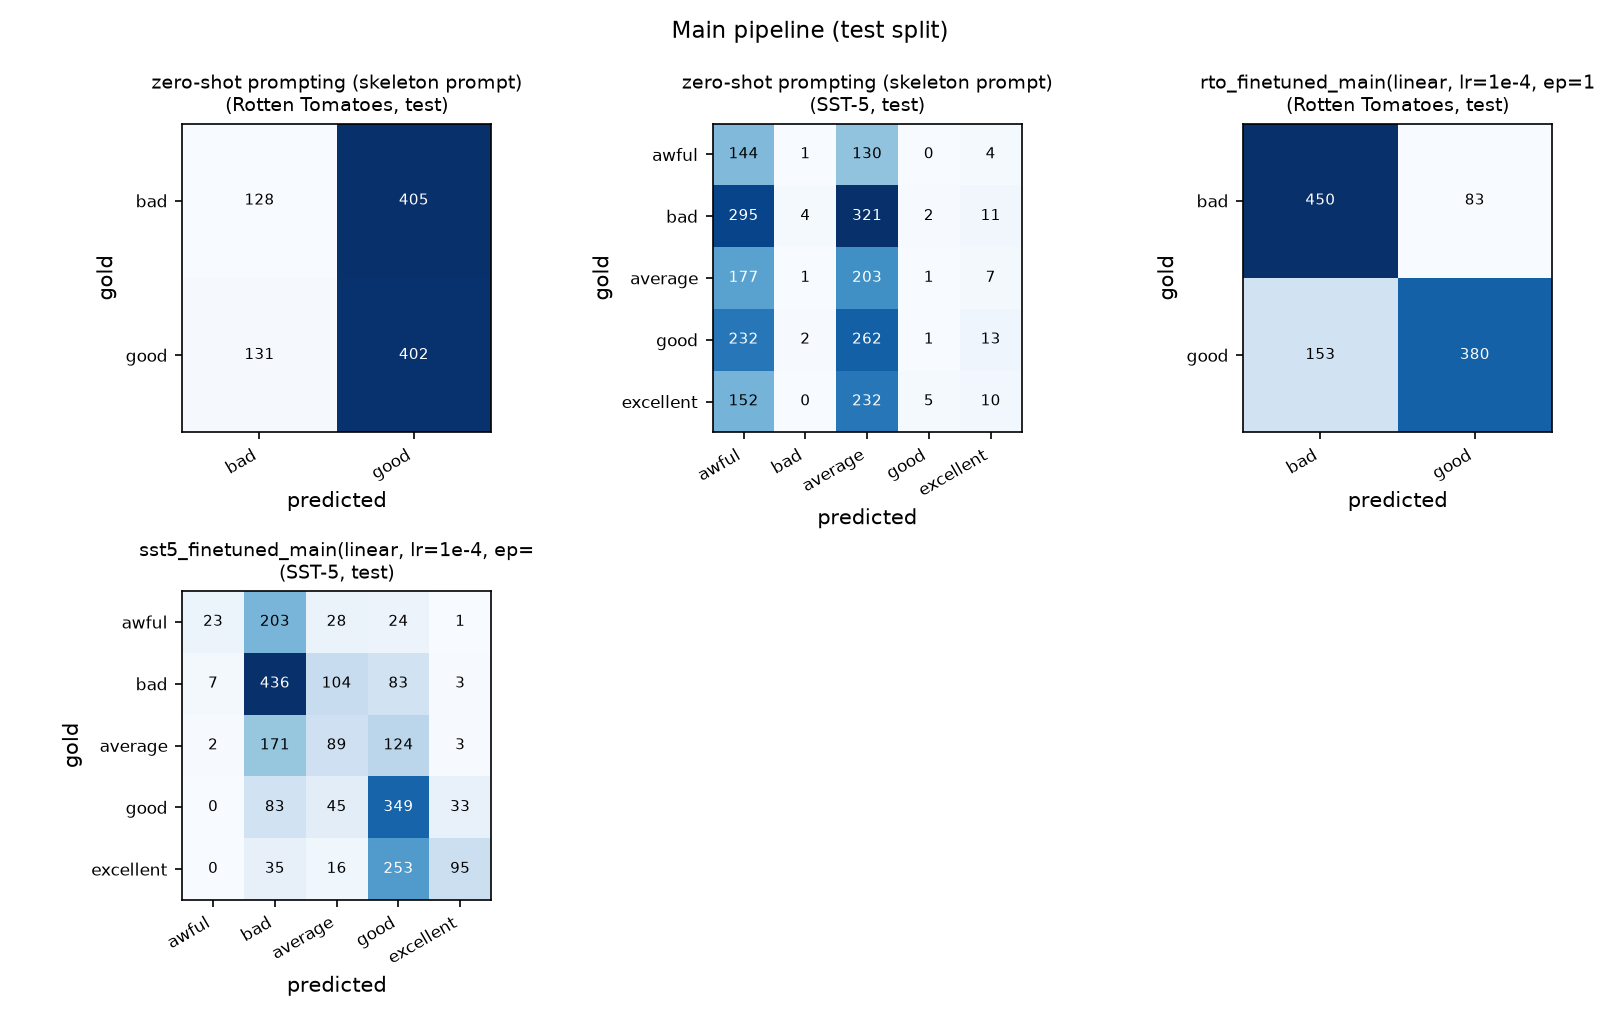
\includegraphics[width=0.75\columnwidth]{figures/confusion_matrices_main.png}
\caption{Test-split confusion matrices for zero-shot prompting and the fine-tuned model on both
datasets (rows: gold labels, columns: predictions); on SST-5 only two classes receive
predictions.}
\label{fig:cm}
\end{figure}

\begin{table}[!ht]
\centering
\setlength{\tabcolsep}{4pt}
\resizebox{\columnwidth}{!}{%
\small
\begin{tabular}{@{}p{1.45in}lccc@{}}
\toprule
Method & Data / split & Acc. & Macro-F1 & F1$_{+}$ \\
\midrule
Zero-shot prompting & RTO / val & 54.97 & 54.87 & 52.76 \\
(skeleton prompt) & RTO / test & 54.03 & 53.98 & 52.33 \\
 & SST-5 / val & 16.26 & 10.34 & -- \\
 & SST-5 / test & 18.46 & 11.72 & -- \\
\addlinespace
Fine-tuned & RTO / val & 76.27 & 76.22 & 75.22 \\
(linear head, lr $10^{-4}$, 1 epoch) & RTO / test & 77.86 & 77.77 & 76.31 \\
 & SST-5 / val & 45.96 & 40.20 & -- \\
 & SST-5 / test & 44.89 & 36.95 & -- \\
\bottomrule
\end{tabular}}
\caption{Main results (\%). F1$_{+}$ is the positive-class F1 (binary task only); for SST-5 the
skeleton's F1 already is the macro average. Source:
\texttt{artifacts/all\_experiment\_metrics.csv}.}
\label{tab:main}
\end{table}

\subsection{Prompt design}
\label{sec:prompts}
The four RTO variants change only the suffix. Test accuracy spans
51.03--57.60\% (53.00--56.85\% on validation) and macro-F1 50.70--56.88\%, and the decision bias
moves with the wording: swapping the label-word order (B) gives the best accuracy and macro-F1
(57.60\%/56.88\%) with 62.9\% positive predictions, the \emph{``\ldots negative or positive?
\ldots''} suffix (C) is worst on both (51.03\%/50.70\%), and a minimal single-label-word suffix
(D) sits in between (54.97\%/54.97\%). Rows 1 and A use the same wording and differ only in
batch size and execution pass; after the padding fix
(Section~\ref{sec:setup-problems}) they agree to the last decimal, the batch invariance the fix
was meant to buy.

On SST-5 the four suffixes separate much more: test accuracy 13.76--18.46\% and macro-F1
7.62--11.81\%, with the skeleton wording best on both splits (18.46\% test, 16.26\% validation)
and the rating-question variant (D) worst on test (14.03\%), almost all of whose predictions are
\emph{awful} (86.7\%) or \emph{good} (13.1\%). F1 for \emph{bad} and \emph{average} never
exceeds 2.7\%.

\begin{table}[!ht]
\centering
\setlength{\tabcolsep}{4pt}
\resizebox{\columnwidth}{!}{%
\small
\begin{tabular}{@{}p{1.6in}ccc@{}}
\toprule
Prompt suffix (RTO, label words in order) & Acc. & Macro-F1 & Pos.\% \\
\midrule
Is this movie bad or good? This movie is (bs 32) & 54.03 & 53.98 & 46.4 \\
A: same wording, second pass (bs 64) & 54.03 & 53.98 & 46.4 \\
B: \ldots good or bad? \ldots & 57.60 & 56.88 & 62.9 \\
C: \ldots negative or positive? The sentiment is & 51.03 & 50.70 & 58.3 \\
D: Overall, this movie is & 54.97 & 54.97 & 49.2 \\
\bottomrule
\end{tabular}}
\caption{Rotten Tomatoes test results for the prompt variants (\%). Pos.\% is the share of
positive predictions; rows 1 and A use the same wording and differ only in batch size and the
execution pass, and now agree exactly, which is the batch-invariance check for the padding fix of
Section~\ref{sec:setup-problems}. SST-5 variants are summarised in the text. Source:
\texttt{artifacts/task1\_prompt\_variants.csv}.}
\label{tab:prompts}
\end{table}

\subsection{Which fine-tuning choices matter}
Table~\ref{tab:ft} varies one training factor at a time on RTO. Epochs matter more than the
learning rate: halving the rate to $5\times10^{-5}$ leaves test accuracy essentially unchanged
(78.80\%, a gap inside the run-to-run variation of Section~\ref{sec:caveats}), while a second
epoch at $10^{-4}$ gives the best result of the study (79.92\% accuracy, 79.90\% macro-F1) for
roughly 1.7 times the training time (1{,}009.6\,s against 600.4\,s). Head capacity adds little:
a 256-dimensional MLP head reaches 79.74\% and a hidden-size MLP head drops to 77.77\%, so added
capacity starts to over-fit the $\sim$8.5k training examples. Linear probing is the most
informative result: freezing the encoder and training only a 1{,}024-parameter classifier
(0.0025\% of the model) already reaches 63.32\% test accuracy, 39.0\% of the gap between
zero-shot prompting and full fine-tuning, and it trains 3.6$\times$ faster (165.5\,s). Most of the benefit of fine-tuning therefore comes from
adapting the pre-trained representation rather than from a stronger classifier, in line with
feature-based and parameter-efficient adaptation
\citep{peters-etal-2018-deep,devlin-etal-2019-bert,li-liang-2021-prefix,lester-etal-2021-power,gao-etal-2021-making}.

\begin{table}[!ht]
\centering
\setlength{\tabcolsep}{4pt}
\resizebox{\columnwidth}{!}{%
\small
\begin{tabular}{@{}p{1.5in}lrrr@{}}
\toprule
Configuration (RTO test split) & Trainable & Train (s) & Acc. & Macro-F1 \\
\midrule
Linear, lr $10^{-4}$, 1 epoch (main) & 41.7M & 600.4 & 77.86 & 77.77 \\
Linear, lr $5\times10^{-5}$, 1 epoch & 41.7M & 506.0 & 78.80 & 78.76 \\
Linear, lr $10^{-4}$, 2 epochs & 41.7M & 1009.6 & \textbf{79.92} & \textbf{79.90} \\
MLP-256 head, 1 epoch & 41.8M & 495.5 & 79.74 & 79.67 \\
MLP-hidden head, 1 epoch & 42.0M & 495.9 & 77.77 & 77.68 \\
Linear probing (encoder frozen) & 1{,}024 & 165.5 & 63.32 & 63.30 \\
\bottomrule
\end{tabular}}
\caption{Fine-tuning variants on Rotten Tomatoes (\%). Validation accuracy is in the text;
``Trainable'' is the number of parameters updated, rounded to 0.1M (exact counts in
Section~2.1). Source: \texttt{artifacts/all\_experiment\_metrics.csv}.}
\label{tab:ft}
\end{table}

\section{Discussion: what drives prompting and fine-tuning performance}

\textbf{Backbone scale and domain.} The checkpoint is small and was pre-trained on stories, not
on reviews, so its zero-shot label-word distribution is dominated by priors over the label words
themselves: on RTO it barely clears chance and leans slightly negative (46.4\% positive
predictions), and on SST-5 it produces only the two extreme adjectives. Prompt engineering can
re-weight such a prior---our best wording recovers 2.90 macro-F1 points on RTO---but it cannot
create sentiment knowledge that is not there:
no SST-5 suffix gets past 18.5\% accuracy, while fine-tuning reaches 44.89\%.

\textbf{Label space and task granularity.} RTO has a symmetric two-word label space, so accuracy
stays in a narrow 51--58\% band for every wording and the larger visible effect of prompting is a
shift in the decision threshold (46--63\% positive predictions) rather than in accuracy. SST-5 asks for a graded judgement whose label words
are not symmetric in frequency or usage and offers no natural answer slot for intensity, so the
model hedges towards \emph{average}.

\textbf{Training budget.} On RTO the one-epoch configurations span less than two accuracy
points (77.77--79.74\%) and only the number of epochs clearly exceeds the run-to-run variation;
the task looks close to what this backbone can do (79.92\%). On SST-5 the ceiling is set by
granularity, not by the prompt: 77.2\% of the errors are between neighbouring classes.

\textbf{Protocol caveats.} Every configuration was run once with one seed, so differences below
about one accuracy point should not be interpreted; all numbers come from the submitted
notebook. Re-executing it in
the same environment reproduces the saved predictions (\texttt{results/*.txt}) byte for byte and
32 of the 34 metric rows in \texttt{artifacts/all\_experiment\_metrics.csv} exactly; in the
remaining configuration (\texttt{rto\_ft\_lr1e-04\_ep2}) accuracy and macro-F1 move by up to 1.2
points between passes, and wall-clock times vary by up to 8\%, so speed differences are
qualitative (``cheaper'', ``$\sim$3.6$\times$ faster'').
\label{sec:caveats} Because prompting and fine-tuning use different batching
(Section~\ref{sec:setup-problems}), I also re-checked that prompting is batch-invariant after the
fix; the prompting numbers above are the corrected ones and are directly comparable across the
batches used here.

\section{Error Analysis}

\subsection{Aggregate behaviour}
Fine-tuned SST-5 makes 1{,}218 errors on 2{,}210 test examples; the statistics below come from
\texttt{artifacts/error\_cases\_*.csv} and the confusion matrices. Of these, 77.2\% are adjacent
(off-by-one) confusions, 17.7\% skip one label, 5.1\% skip two and one error skips three, so the
model orders sentiment correctly even when it misses the exact level. Zero-shot prompting fails
differently: only 37.3\% of its 2{,}724 errors are adjacent, it predicts only the two extreme
labels, and it recovers almost none of the \emph{bad}, \emph{average} and \emph{good} examples
(recall 0.0\%, 0.0\% and 1.4\%).

RTO is skewed in the same direction under both methods. The first 300 zero-shot validation
errors are dominated by false negatives (265 \emph{good}$\rightarrow$\emph{bad} against 35
\emph{bad}$\rightarrow$\emph{good}), and the first 300 errors after fine-tuning (253 from
validation, 47 from test) keep that skew (196 against 104), so fine-tuning only partly corrects
the prompting bias. More than half of the sampled RTO validation errors after fine-tuning
(57.7\%, 146 of 253) were already errors under prompting (75.7\%, 227 of 300, on SST-5
validation), so fine-tuning inherits the prompting errors as well as introducing its own.

\subsection{Case studies}
\textbf{Very short inputs.} The zero-shot model calls \textit{``crummy''} and \textit{``terrible
.''} (gold \emph{bad}) positive: with one or two tokens there is no context to accumulate
evidence, so the label-word prior decides.

\textbf{Implicit sentiment.} After fine-tuning, \textit{``a well-executed spy-thriller .''} and
\textit{``[a] satisfying niblet .''} (gold \emph{good}) are labelled \emph{bad}, matching the
false-negative skew above: praise expressed through a noun phrase or a fragment is not captured.

\textbf{Negation and intensity.} \textit{``i do n't think i laughed out loud once .''} (gold
\emph{awful}) is predicted \emph{bad}, and \textit{``lovely and poignant .''} (gold
\emph{excellent}) is predicted \emph{good}: polarity survives but intensity is compressed
towards the middle. In each 300-error sample, an explicit negation token appears in 20.7\% (62/300) and 23.3\% (70/300) of
the fine-tuned RTO and SST-5 error sets against 17.0\% (51/300) and 21.7\% (65/300) zero-shot, so
fine-tuning does not remove negation-adjacent errors (notebook cell 83).

\textbf{No cue at all.} \textit{``that 's a cheat .''} (gold \emph{bad}) is predicted
\emph{average}: with no sentiment word present, the model falls back on the middle
class.

\subsection{Bottlenecks and what we would improve}
The extreme classes are effectively unsolved: recall is 8.2\% for \emph{awful} and 23.8\% for
\emph{excellent} against 68.9\% for \emph{bad} and 68.4\% for \emph{good}, so the strongest and
weakest opinions are softened most often. An ordinal objective, or a regression head
over the five ordered levels with label smoothing across neighbours, would target exactly the
77.2\% adjacent-error mass. Capacity is the second constraint: a 1{,}024-parameter classifier
captures 39.0\% of the fine-tuning gain but is capped at 63.32\%. Sentiment-specific
calibration---subtracting the model's prior over the label words or adding in-context
demonstrations---is the cheapest next experiment.

\section{Conclusion}
Zero-shot label-word prompting of a 42M-parameter story model is barely above chance on binary
sentiment and nearly unusable on SST-5: prompt wording can re-balance the output but
cannot supply sentiment knowledge the model never had. Fine-tuning the same model reaches
77.86\% test accuracy on Rotten Tomatoes and 44.89\% on SST-5, and a head-only classifier with
1{,}024 parameters already recovers 39.0\% of the distance from prompting to full fine-tuning.
What remains is concentrated at the extremes and between neighbouring classes of the graded
task, and that is where I would spend the next training budget: an ordinal objective, and a
larger backbone.

\section*{Use of Generative AI}
I acknowledge the use of DeepSeek (\url{https://www.deepseek.com}) for explaining concepts,
suggesting hints and ideas, debugging and rewriting code, and giving feedback on drafts; I did
not use it to generate a complete solution or to copy its answers directly, and the report text
is my own. All experiments were run end to end on my local machine, and every number, table and
figure comes from that execution and was verified against the saved outputs
(\texttt{results/*.txt}, \texttt{artifacts/}), with nothing fabricated, altered or estimated by
an AI system.

{\footnotesize
\bibliography{custom}
}

\end{document}
